\begin{figure}
    \centering
    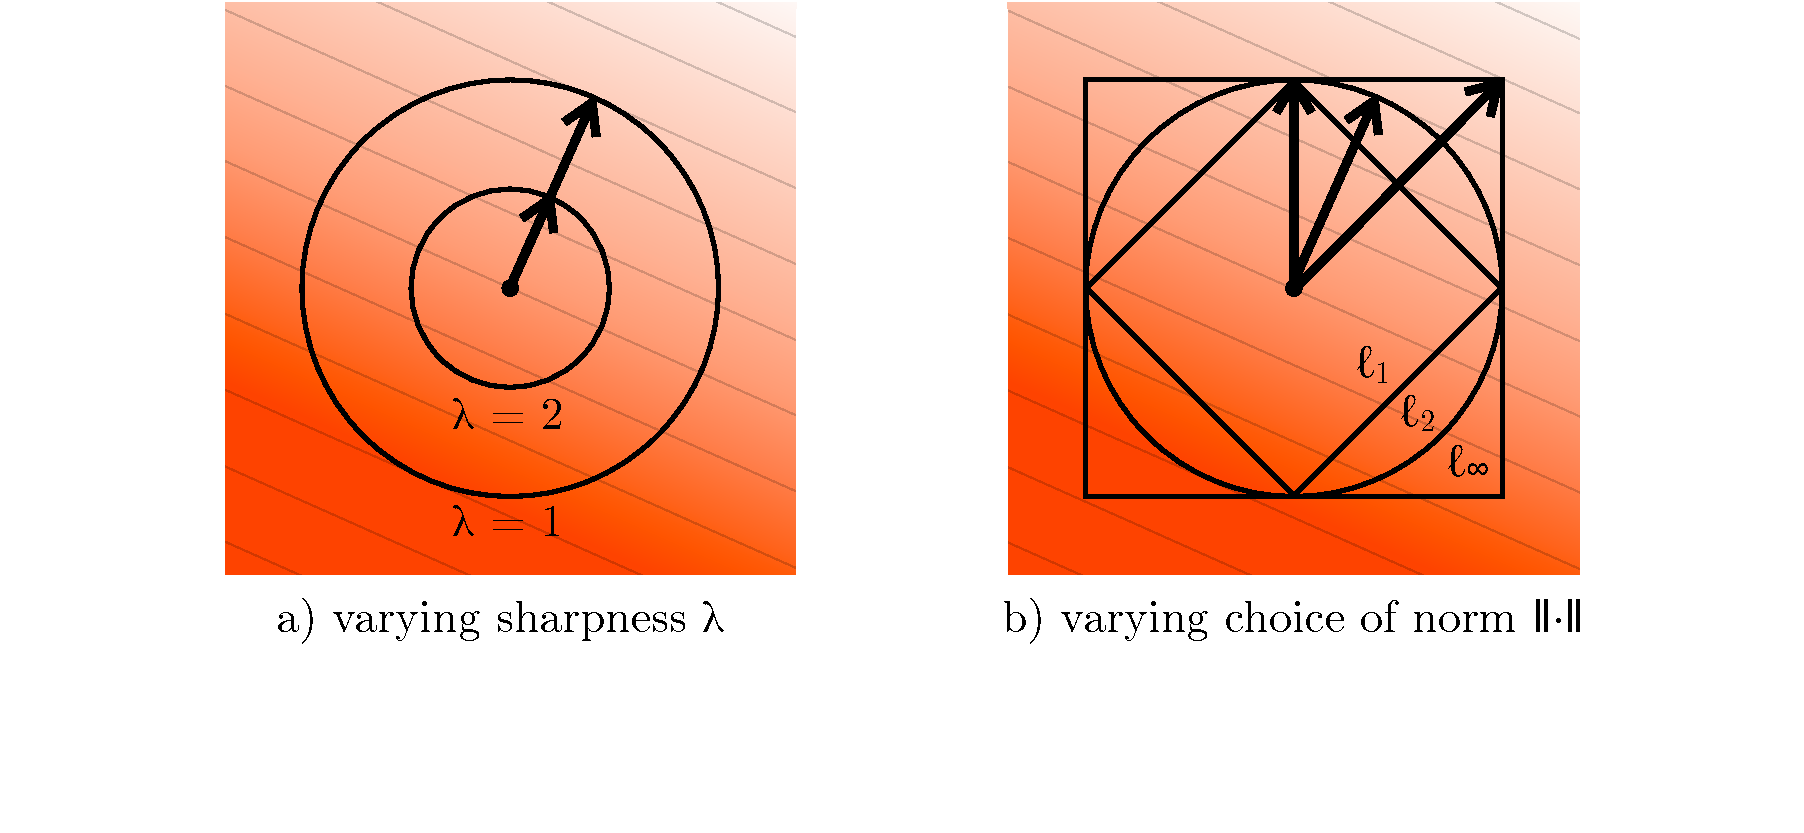
\includegraphics[width=\linewidth,trim={0 3.2cm 0 0},clip]{figure/norms}
    \vspace{-1em}
    \caption{Steepest descent considers the problem of minimizing a linear functional under a quadratic penalty: $\argmin_{\Delta \vw \in \R^n} \left[\vg^\top \Delta \vw + \frac{\lambda}{2} \, \norm{\Delta \vw}^2 \right]$ for $\vg \in \R^n$. Here we show how the solution varies with the sharpness $\lambda > 0$ and the choice of norm $\norm{\cdot}$. We overlay different norm balls on top of a linear color gradient, and use arrows to denote the solution, meaning the member of the norm ball that ``minimizes the color''. a) Increasing the sharpness decreases the size of the solution vector. b) Changing the norm can change the direction of the solution vector. For different $\ell_p$ norms, the solution direction changes because the gradient is not axis-aligned. In practice, we should pick the sharpness and norm to fit the geometry of our loss.}
    \label{fig:contours}
\end{figure}
